\documentclass[aspectratio=169,10pt]{beamer}

\usetheme{Madrid}
\usecolortheme{default}
\setbeamertemplate{navigation symbols}{}
\setbeamertemplate{bibliography item}{\insertbiblabel}

\usepackage[utf8]{inputenc}
\usepackage[T1]{fontenc}
\usepackage{amsmath,amssymb,amsfonts}
\usepackage{booktabs}
\usepackage{tikz}
\usetikzlibrary{arrows.meta,positioning,calc}
\usepackage{pgfplots}
\pgfplotsset{compat=1.16}
\usepackage{listings}
\lstset{language=Python,basicstyle=\ttfamily\scriptsize,keywordstyle=\color{blue!60!black},
        commentstyle=\color{black!55},showstringspaces=false,columns=fullflexible,
        backgroundcolor=\color{black!4},frame=single,framerule=0pt,xleftmargin=0pt}

% ---------- macros ----------
\newcommand{\dd}{\mathrm{d}}
\newcommand{\ii}{\mathrm{i}}
\newcommand{\ee}{\mathrm{e}}
\newcommand{\bq}{\mathbf{q}}
\newcommand{\LL}{\mathcal{L}}   % fast (acoustic) operator
\newcommand{\NN}{\mathcal{N}}   % slow (advective) operator
\newcommand{\ph}{\varphi}

\title[Acoustics with advection]{Linear Acoustics with Advection\\and Multirate Time Integration}
\subtitle{Split-explicit, exponential, Lawson, averaging and resonance-based methods}
\author{Your Name}
\institute[]{Your Institute}
\date{\today}

\begin{document}

% =====================================================================
\begin{frame}
  \titlepage
\end{frame}

\begin{frame}{Outline}
  \tableofcontents
\end{frame}

% =====================================================================
\section{Motivation: time integration in NWP}
% =====================================================================

\begin{frame}{Why this problem? Time stepping in numerical weather models}
  \begin{itemize}
    \item Compressible (non-hydrostatic) dynamical cores solve the Euler equations on the sphere/in a box.
    \item Wide range of time scales in one system:
    \begin{center}
    \begin{tabular}{lcc}
      \toprule
      process & speed & role\\
      \midrule
      sound waves & $c\approx 340\,\mathrm{m/s}$ & fast, \emph{not} meteorologically relevant\\
      gravity waves & $\sim 30$--$100\,\mathrm{m/s}$ & fast/intermediate\\
      advection by wind & $U\approx 10$--$50\,\mathrm{m/s}$ & slow, \emph{relevant}\\
      \bottomrule
    \end{tabular}
    \end{center}
    \item Fully explicit methods: step size limited by $c\,\Delta t/\Delta x \lesssim 1$ \;$\Rightarrow$\; far smaller than accuracy needs for the slow, relevant dynamics.
    \item Fully implicit: global (Helmholtz-type) solves, poor scalability on massively parallel machines.
  \end{itemize}
  \vspace{0.5em}
  \begin{alertblock}{Key idea}
    Treat the fast part cheaply/exactly and the slow part with a large step: \textbf{multirate / split / exponential} methods.
  \end{alertblock}
\end{frame}

\begin{frame}{Where it is used and what is needed}
  \begin{itemize}
    \item Split-explicit time stepping (Klemp--Wilhelmson; Wicker--Skamarock RK3 with acoustic substeps) is the standard in WRF, COSMO/ICON-type and many other cores.
    \item Exponential integrators and multirate schemes are active research directions for dynamical cores.
    \item The \textbf{linear acoustic--advection system} is the core subproblem:
    \begin{itemize}
      \item it contains exactly the scale separation $c \gg U$ (Mach number $M=U/c\approx 0.1$),
      \item it allows analysis in Fourier space (stability, dispersion, resonance),
      \item errors of any scheme for the full nonlinear system must at least be good here.
    \end{itemize}
  \end{itemize}
  \vspace{0.5em}
  \textbf{Plan of the talk}
  \begin{enumerate}
    \item model problem and the abstract splitting $\bq'=\LL\bq+\NN\bq$
    \item split-explicit methods as a special case of ETD
    \item Lawson, averaging and resonance-based methods
    \item application: staggered grids in 1D and 2D with high-order advection
  \end{enumerate}
\end{frame}

% =====================================================================
\section{Model problem}
% =====================================================================

\begin{frame}{Linear acoustics with advection}
  Perturbations $(p,u)$ about a constant background state $(\rho_0,U)$, speed of sound $c$:
  \begin{align*}
    \partial_t u + U\,\partial_x u + \tfrac{1}{\rho_0}\,\partial_x p &= 0,\\
    \partial_t p + U\,\partial_x p + \rho_0 c^2\,\partial_x u &= 0.
  \end{align*}
  Write $\bq=(p,u)^\top$ and split
  \[
    \partial_t \bq = \underbrace{-\begin{pmatrix}0&\rho_0c^2\\ 1/\rho_0&0\end{pmatrix}\partial_x\bq}_{\LL\bq:\ \text{acoustic (fast)}}
                   \;\underbrace{-\,U\,\partial_x\bq}_{\NN\bq:\ \text{advection (slow)}}.
  \]
  \begin{itemize}
    \item $\LL$: eigenvalues in Fourier space $\pm\ii c k$ (purely oscillatory, large).
    \item $\NN$: eigenvalue $-\ii U k$ (small, $|U|\ll c$).
    \item For constant $U$ on a periodic domain the two operators \textbf{commute}, also after discretization with
    the same stencil for $p$ and $u$ (all operators are circulant). Non-commutativity enters via
    variable $U(x)$, boundaries, or flux-form/interpolated discretizations.
  \end{itemize}
\end{frame}

\begin{frame}{Abstract setting}
  \[
    \bq'(t)=\LL\bq(t)+\NN\bq(t),\qquad \bq(t_0)=\bq_0 ,
  \]
  after spatial discretization: $\LL,\NN$ are matrices, $\|h\LL\|\gg\|h\NN\|$ for the time steps of interest.

  \medskip
  \textbf{Variation of constants} over one step $[t_n,t_n+h]$:
  \[
    \bq(t_n+h)=\ee^{h\LL}\bq_n+\int_0^h \ee^{(h-s)\LL}\,\NN\,\bq(t_n+s)\,\dd s .
  \]
  \begin{itemize}
    \item The fast part is treated \emph{exactly} (or very accurately) through $\ee^{h\LL}$.
    \item Only the slow part $\NN\bq$ must be approximated; its time scale is $\sim 1/(Uk)$.
    \item Different multirate methods = different ways to approximate this integral.
  \end{itemize}
  \vspace{0.3em}
  \textbf{Notation:} $\ph_1(z)=\dfrac{\ee^z-1}{z}$, \quad $\ph_2(z)=\dfrac{\ph_1(z)-1}{z}$, \quad $\ph_{k+1}(z)=\dfrac{\ph_k(z)-1/k!}{z}$.
\end{frame}

% =====================================================================
\section{Split-explicit methods as ETD}
% =====================================================================

\begin{frame}{Exponential time differencing (ETD)}
  Approximate $\NN\bq(t_n+s)$ by a polynomial in $s$ and integrate the exponential exactly.

  \medskip
  \textbf{ETD1 (exponential Euler):}
  \[
    \bq_{n+1}=\ee^{h\LL}\bq_n+h\,\ph_1(h\LL)\,\NN\bq_n .
  \]
  \textbf{ETD2 / ETDRK2 (Cox--Matthews type):}
  \begin{align*}
    \mathbf{a}_n &= \ee^{h\LL}\bq_n+h\,\ph_1(h\LL)\NN\bq_n,\\
    \bq_{n+1} &= \mathbf{a}_n + h\,\ph_2(h\LL)\big(\NN\mathbf{a}_n-\NN\bq_n\big).
  \end{align*}
  \begin{itemize}
    \item Exact for $\bq'=\LL\bq+\mathbf{g}$ with constant $\mathbf{g}$ (``frozen slow tendency'').
    \item Requires $\ee^{h\LL}\mathbf{v}$ and $\ph_k(h\LL)\mathbf{v}$: Krylov / Fourier / (rational) approximations.
    \item Acoustic oscillations: no CFL restriction from $c$ at all (but see resonances later).
  \end{itemize}
\end{frame}

\begin{frame}{Split-explicit time stepping}
  Klemp--Wilhelmson / Wicker--Skamarock: freeze the slow tendency during the step and integrate the fast
  system by $m$ small substeps $\tau=h/m$ (forward--backward for the acoustic part):
  \[
    \mathbf{z}_0=\bq_n,\qquad
    \mathbf{z}_{j+1}=\mathbf{z}_j+\tau\big(\LL\mathbf{z}_j+\mathbf{g}\big),\quad \mathbf{g}=\NN\bq_n,
    \qquad \bq_{n+1}=\mathbf{z}_m .
  \]
  Since $\mathbf{z}'=\LL\mathbf{z}+\mathbf{g}$ has the exact solution $\ee^{t\LL}\bq_n+t\,\ph_1(t\LL)\mathbf{g}$,
  \begin{align*}
    \mathbf{z}_m &= (I+\tau\LL)^m\bq_n+\tau\sum_{j=0}^{m-1}(I+\tau\LL)^j\,\mathbf{g}\\
                 &\approx \ee^{h\LL}\bq_n + h\,\ph_1(h\LL)\mathbf{g}.
  \end{align*}
  \begin{block}{Split-explicit $=$ ETD1 with substepped approximations}
    $\ee^{h\LL}\;\to\;R_m(\tau\LL)=(I+\tau\LL)^m$ and $\ph_1(h\LL)\;\to\;\frac1m\sum_{j<m}(I+\tau\LL)^j$.
    The same view applies to the RK3 outer loop of Wicker--Skamarock (stages with $h/3,\,h/2,\,h$).
  \end{block}
\end{frame}

\begin{frame}{Consequences of the ETD view}
  \begin{itemize}
    \item \textbf{Order:} the slow forcing is frozen $\Rightarrow$ first order for the pure ETD1 version; higher order
    through RK-type outer stages or ETDRK schemes with $\ph_2,\ph_3$.
    \item \textbf{Fast part inexact:} $\ee^{h\LL}$ is replaced by a stability-limited polynomial; the substep count $m$
    controls both accuracy and stability (acoustic Courant number $c\tau/\Delta x\le C$).
    \item \textbf{Free choice of ``fast solver''}: substepping, Fourier/FFT (periodic), Krylov, Chebyshev --
    all realize the same ETD framework.
    \item \textbf{Analysis in Fourier space:} on each mode, $\LL\to\pm\ii ck$, $\NN\to-\ii Uk$ and
    all $\ph_k(\ii\theta)$ with $\theta=\pm ckh$ are explicit; amplification factors can be compared with
    $\ee^{-\ii (\pm c-U)\,kh}$.
  \end{itemize}
\end{frame}

% =====================================================================
\section{Lawson, averaging and resonance methods}
% =====================================================================

\begin{frame}{Lawson (integrating factor) methods}
  Change variables $\mathbf{v}(t)=\ee^{-(t-t_n)\LL}\bq(t)$:
  \[
    \mathbf{v}'(t)=\ee^{-(t-t_n)\LL}\,\NN\,\ee^{(t-t_n)\LL}\mathbf{v}(t)=:\widetilde\NN(t)\,\mathbf{v}(t),
  \]
  \textbf{apply an explicit Runge--Kutta method to $\mathbf{v}$} and transform back.

  \medskip
  \textbf{Lawson--Euler:}
  \[
    \bq_{n+1}=\ee^{h\LL}\big(\bq_n+h\,\NN\bq_n\big).
  \]
  \textbf{Lawson--RK4:} classical RK4 with $\ee^{c_ih\LL}$ weights, e.g.\ stage values
  $\mathbf{Y}_i=\ee^{c_ih\LL}\bq_n+h\sum_j a_{ij}\,\ee^{(c_i-c_j)h\LL}\NN\mathbf{Y}_j$.
  \begin{itemize}
    \item Simple to implement: only matrix exponentials of $\LL$ (diagonal in Fourier space).
    \item Order conditions are those of the underlying RK method (for sufficiently smooth solutions).
    \item Drawbacks: does not preserve steady states of $\LL+\NN$; error constants depend on $\|\NN\|$, not on a
    well-adapted $\ph$-function structure; stiff order reduction possible.
  \end{itemize}
\end{frame}

\begin{frame}{Efficient Lawson-RK4}
  Classical RK4 on $\mathbf{v}'=\widetilde\NN(t)\mathbf{v}$ with $E=\ee^{h\LL/2}$ gives
  \[
    \bq_{n+1}=E^2\bq_n+\tfrac h6\big(E^2\mathbf{k}_1+2E(\mathbf{k}_2+\mathbf{k}_3)+\mathbf{k}_4\big),
  \]
  with stages $\mathbf{Y}_1=\bq_n$, $\mathbf{Y}_2=E(\bq_n+\tfrac h2\mathbf{k}_1)$, $\mathbf{Y}_3=E\bq_n+\tfrac h2\mathbf{k}_2$,
  $\mathbf{Y}_4=E^2\bq_n+hE\mathbf{k}_3$, \; $\mathbf{k}_i=\NN\mathbf{Y}_i$.

  \medskip
  \textbf{Reorganized with $E$ applied to sums} (using linearity of $E$):
  \begin{align*}
    \mathbf{k}_1&=\NN\bq_n, & \mathbf{w}&=E\bq_n, & \mathbf{Y}_2&=E\big(\bq_n+\tfrac h2\mathbf{k}_1\big), & \mathbf{k}_2&=\NN\mathbf{Y}_2,\\
    \mathbf{Y}_3&=\mathbf{w}+\tfrac h2\mathbf{k}_2, & \mathbf{k}_3&=\NN\mathbf{Y}_3, & \mathbf{Y}_4&=E\big(\mathbf{w}+h\mathbf{k}_3\big), & \mathbf{k}_4&=\NN\mathbf{Y}_4,
  \end{align*}
  \[
    \bq_{n+1}=E\Big[\mathbf{w}+\tfrac13\big(\mathbf{Y}_2-\mathbf{w}\big)+\tfrac h3(\mathbf{k}_2+\mathbf{k}_3)\Big]+\tfrac h6\mathbf{k}_4 .
  \]
  \begin{itemize}
    \item \textbf{4 evaluations of $\NN$ and 4 applications of $E$} per step; $\ee^{h\LL}=E^2$ is never formed
    ($\tfrac13(\mathbf{Y}_2-\mathbf{w})=\tfrac h6E\mathbf{k}_1$ reuses $\mathbf{Y}_2$).
    \item $E$ is precomputed once: on the staggered grid a $2\times2$ block per wavenumber, applied by FFT.
  \end{itemize}
\end{frame}

\begin{frame}{Averaging methods}
  \textbf{Observation:} in the interaction picture the slow forcing is
  \[
    \widetilde\NN(s)=\ee^{-s\LL}\NN\,\ee^{s\LL},
  \]
  which oscillates with the fast (acoustic) frequencies $\pm ck$.
  Its time average
  \[
    \overline{\NN}_h=\frac1h\int_0^h \ee^{-s\LL}\NN\,\ee^{s\LL}\,\dd s
  \]
  carries the net slow effect; oscillating contributions average out.

  \medskip
  \textbf{Averaged integrator} (first order sketch):
  \[
    \bq_{n+1}=\ee^{h\LL}\Big(I+h\,\overline{\NN}_h\Big)\bq_n \quad\text{or}\quad \bq_{n+1}=\ee^{h(\LL+\overline{\NN}_h)}\bq_n .
  \]
  \begin{itemize}
    \item For commuting $\LL,\NN$: $\overline{\NN}_h=\NN$, and the scheme is exact in the continuum.
    \item For non-commuting operators (variable wind, interpolated fluxes, boundaries), $\overline{\NN}_h$ captures the leading
    commutator corrections $[\LL,\NN]$.
    \item The average can be computed by quadrature in $s$, by a Fourier/eigenbasis formula, or by substeps.
  \end{itemize}
\end{frame}

\begin{frame}{Resonances}
  On a Fourier mode with $\LL\to\pm\ii\omega$, $\omega=ck$, the exponential integrator terms contain
  \[
    \ph_1(\ii\theta)=\frac{\ee^{\ii\theta}-1}{\ii\theta},\qquad \theta=\omega h,
  \]
  and error constants contain factors like $1/\sin(\theta/2)$ in multistep/mean-value type schemes.

  \medskip
  \begin{alertblock}{Step-size resonances}
    When $\omega h\approx 2\pi n$ (the step is a multiple of the acoustic period), errors can be amplified
    (in the worst case, instability) for some exponential/Lawson schemes.
  \end{alertblock}
  \textbf{Resonance-based (filtered) methods:}
  \begin{itemize}
    \item expand the Duhamel integral and integrate the oscillatory factors $\ee^{\ii s(\pm\omega_1\pm\omega_2)}$ \emph{exactly};
    \item resonant combinations ($\omega_1\pm\omega_2\approx0$) are kept as they are, non-resonant ones are integrated analytically;
    \item result: error bounds that do not depend on $\omega h$ and no step-size resonance.
  \end{itemize}
\end{frame}

\begin{frame}{Comparison of the schemes (what we will test)}
  \centering
  \begin{tabular}{lccc}
    \toprule
     & fast part & slow part & resonance\\
    \midrule
    split-explicit     & substepped polynomial  & frozen / RK stages & none (stability limit)\\
    ETD(RK)            & exact $\ee^{h\LL}$, $\ph_k$ & polynomial in $s$ & possible\\
    Lawson             & exact $\ee^{h\LL}$     & RK on interaction picture & possible\\
    averaging          & exact $\ee^{h\LL}$     & time-averaged $\overline\NN_h$ & reduced\\
    resonance-based    & exact $\ee^{h\LL}$     & oscillatory integrals exact & avoided\\
    \bottomrule
  \end{tabular}
  \medskip
  \begin{itemize}
    \item Criteria: order in $h$, accuracy vs.\ $\omega h$ (large acoustic steps), cost (number of $\LL$-evaluations / FFTs / substeps),
    robustness near $ckh=2\pi n$.
  \end{itemize}
\end{frame}

% =====================================================================
\section{Application: staggered grids, high-order advection}
% =====================================================================

\begin{frame}{Spatial discretization: staggered grid (1D)}
  \begin{center}
  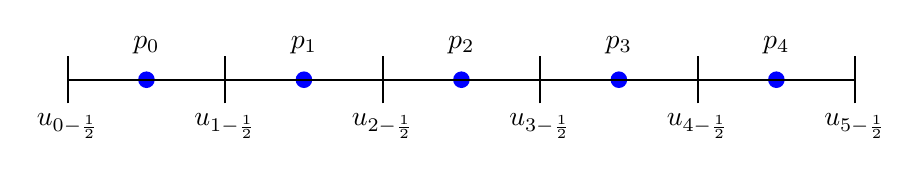
\begin{tikzpicture}[scale=1.0]
    \foreach \i in {0,...,5}{
      \draw[thick] (2*\i,-0.3) -- (2*\i,0.3);
      \node[below] at (2*\i,-0.3) {$u_{\i-\frac12}$};
    }
    \foreach \i in {0,...,4}{
      \fill[blue] (2*\i+1,0) circle (3pt);
      \node[above] at (2*\i+1,0.2) {$p_{\i}$};
    }
    \draw[thick] (0,0) -- (10,0);
  \end{tikzpicture}
  \end{center}
  \begin{itemize}
    \item $p$ at cell centers, $u$ at cell faces (Arakawa C in 2D): compact, accurate acoustic operator
    \[
      (\partial_x u)_j\approx\frac{u_{j+1/2}-u_{j-1/2}}{\Delta x},\qquad
      (\partial_x p)_{j+1/2}\approx\frac{p_{j+1}-p_j}{\Delta x}\quad(\text{2nd order}).
    \]
    \item Higher order: wider centered staggered stencils (4th/6th order) for $\LL$.
    \item \textbf{Advection} $\NN=-U\partial_x$: both fields must be advected on their own grid points
    $\Rightarrow$ high-order upwind-biased stencils (e.g.\ 3rd/5th order). With constant $U$ and the same stencil on both
    arrays, $\LL$ and $\NN$ are circulant and commute: the exact semi-discrete solution is known (used as reference below).
  \end{itemize}
\end{frame}

\begin{frame}{High-order advection operators}
  Upwind-biased reconstruction of face values $\hat\phi_{j+1/2}$ (for $U>0$), advective operator
  \[
    (\NN\phi)_j=-\frac{U}{\Delta x}\big(\hat\phi_{j+1/2}-\hat\phi_{j-1/2}\big).
  \]
  \begin{center}
  \begin{tabular}{ll}
    \toprule
    order & face reconstruction \\
    \midrule
    1st & $\hat\phi_{j+1/2}=\phi_j$\\
    3rd & $\hat\phi_{j+1/2}=\tfrac16\big(-\phi_{j-1}+5\phi_j+2\phi_{j+1}\big)$\\
    5th & $\hat\phi_{j+1/2}=\tfrac1{60}\big(2\phi_{j-2}-13\phi_{j-1}+47\phi_j+27\phi_{j+1}-3\phi_{j+2}\big)$\\
    \bottomrule
  \end{tabular}
  \end{center}
  \begin{itemize}
    \item Odd orders: built-in dissipation (upwinding) $\Rightarrow$ implicit damping of grid-scale noise.
    \item Time integrator error must stay below the spatial error: low-order splitting would spoil the high-order advection.
    \item Fourier symbol of the discrete operator: $\NN\to-\ii U\,\kappa(k\Delta x)/\Delta x$, used for analysis of all schemes above.
  \end{itemize}
\end{frame}

\begin{frame}{Test setup: 1D}
  \begin{itemize}
    \item Periodic domain $[0,L]$, background $U$, $c$ with $M=U/c\in\{0.05,0.1,0.3\}$.
    \item Smooth initial data: Gaussian pressure pulse (right/left moving acoustic waves + advection).
    \item Reference: exact solution (analytic in Fourier space) / very fine time step.
    \item Study:
    \begin{enumerate}
      \item convergence in $h$ for each scheme (fixed fine grid),
      \item error vs.\ acoustic Courant number $c\,h/\Delta x$ up to $\gg1$,
      \item behaviour near resonance $ckh=2\pi n$,
      \item work--precision (number of evaluations of $\LL$, $\NN$, or substeps).
    \end{enumerate}
  \end{itemize}
\end{frame}

\begin{frame}[fragile]{Lawson-RK4 on the staggered grid: code}
\begin{lstlisting}
def E(p, u):                       # apply exp(h/2 L), one 2x2 block per wavenumber
    ph, uh = rfft(p), rfft(u)      # C, aS, bS: precomputed (cos, sin/omega)
    return irfft(C*ph + aS*uh, nx), irfft(bS*ph + C*uh, nx)

def step(p, u):                    # 4 evaluations of N, 4 applications of E
    ap, au = N(p), N(u)                                   # k1
    wp, wu = E(p, u)                                      # w = E y
    y2p, y2u = E(p + h/2*ap, u + h/2*au)                  # Y2
    bp, bu = N(y2p), N(y2u)                               # k2
    cp, cu = N(wp + h/2*bp), N(wu + h/2*bu)               # k3   (Y3 = w + h/2 k2)
    y4p, y4u = E(wp + h*cp, wu + h*cu)                    # Y4
    dp, du = N(y4p), N(y4u)                               # k4
    sp = wp + (y2p - wp)/3 + h/3*(bp + cp)
    su = wu + (y2u - wu)/3 + h/3*(bu + cu)
    sp, su = E(sp, su)
    return sp + h/6*dp, su + h/6*du
\end{lstlisting}
  \vspace{-0.3em}
  \begin{itemize}\footnotesize
    \item $N$: 5th order upwind flux (\texttt{np.roll}, real space), $E$: 4th order staggered acoustic operator, exact exponential.
    \item Checked against a naive Lawson-RK4 (8 exponentials): identical to round-off.
  \end{itemize}
\end{frame}

\begin{frame}{1D experiment: pressure pulse}
  \footnotesize
  $c=350$\,m/s, $U=50$\,m/s ($M=1/7$), $L=1000$\,km, 400 cells, $T=10^4$\,s: $(c+U)T=4L$ and $(c-U)T=3L$,
  so both acoustic pulses return to the start. Initial $p$: Gaussian, $u=0$. $h=50$\,s: $ch/\Delta x=7$, $Uh/\Delta x=1$.
  \begin{center}
    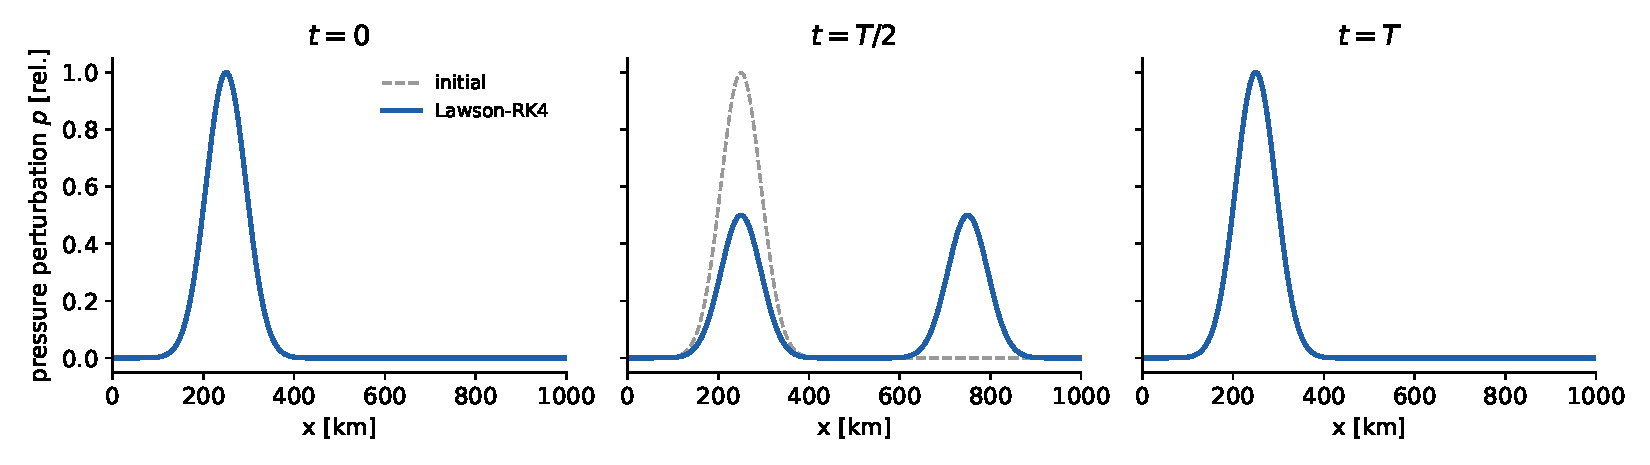
\includegraphics[width=\textwidth]{fig_pressure_1d.pdf}
  \end{center}
  \begin{itemize}
    \item $t=T/2$: the pulse has split into two half-amplitude pulses; the right-going one has traveled $2L$, the left-going one $1.5L$.
    \item $t=T$: back at the initial position; max.\ deviation $6\cdot10^{-6}$ (spatial dissipation of the upwind stencil plus time error).
  \end{itemize}
\end{frame}

\begin{frame}{1D experiment: convergence of Lawson-RK4}
  \begin{columns}[T]
    \column{0.55\textwidth}
      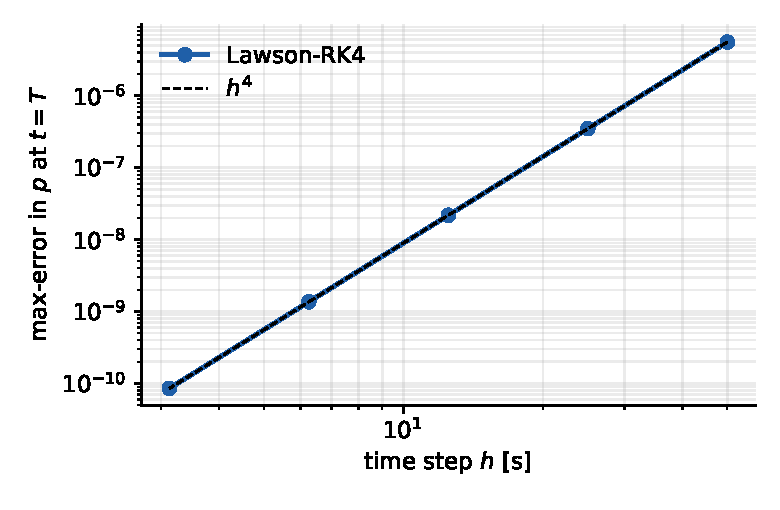
\includegraphics[width=\textwidth]{fig_convergence_1d.pdf}
    \column{0.43\textwidth}
      \footnotesize
      \begin{itemize}
        \item Error against the exact semi-discrete solution at $t=T$.
        \item Observed order $4.00$ for $h=50$\,s down to $3$\,s (acoustic Courant number $7\to0.4$).
        \item Here $\LL$ and $\NN$ commute, so the interaction-picture solution is $\ee^{t\NN}\bq_0$ and the error does not grow with $c$ (same max-error for $c=350$ and $700$\,m/s).
        \item Next: variable wind $U(x)$ and 2D, where $[\LL,\NN]\neq0$.
      \end{itemize}
  \end{columns}
\end{frame}

\begin{frame}{Two dimensions}
  \[
    \partial_t\!\begin{pmatrix}p\\u\\v\end{pmatrix}
    =-\begin{pmatrix}\rho_0c^2(\partial_xu+\partial_yv)\\ \tfrac1{\rho_0}\partial_xp\\ \tfrac1{\rho_0}\partial_yp\end{pmatrix}
     -\big(U\partial_x+V\partial_y\big)\begin{pmatrix}p\\u\\v\end{pmatrix}.
  \]
  \begin{center}
  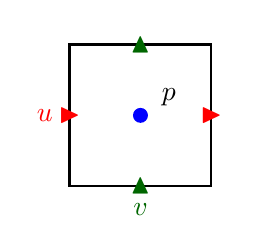
\begin{tikzpicture}[scale=0.9]
    \draw[thick] (0,0) rectangle (2,2);
    \fill[blue] (1,1) circle (3pt); \node at (1.4,1.25) {$p$};
    \node[red] at (0,1) {$\blacktriangleright$}; \node[red,left] at (-0.1,1) {$u$};
    \node[red] at (2,1) {$\blacktriangleright$};
    \node[black!60!green] at (1,0) {$\blacktriangle$}; \node[black!60!green,below] at (1,-0.1) {$v$};
    \node[black!60!green] at (1,2) {$\blacktriangle$};
  \end{tikzpicture}
  \end{center}
  \begin{itemize}
    \item Arakawa C-grid: $p$ at centers, $u$ on vertical faces, $v$ on horizontal faces.
    \item Advection of $u$ and $v$ requires \emph{different} stencils in $x$ and $y$; high-order upwind per direction.
    \item Fast operator $\LL$: 2D wave operator; $e^{h\LL}$ via FFT (periodic) or substepping.
    \item Tests: acoustic pulse in a uniform wind $(U,V)$; rotated wind to test directional splitting errors.
  \end{itemize}
\end{frame}

\begin{frame}{Expected observations (hypotheses to check)}
  \begin{itemize}
    \item Split-explicit: simple, but accuracy limited by frozen slow forcing; error scales with the substep count and the
    acoustic Courant number.
    \item ETD/Lawson: acoustic stability for arbitrary $h$, order determined by the outer RK/ETD scheme.
    \item Resonance steps $ckh\approx 2\pi n$: visible spikes in the error for Lawson/ETD; reduced for averaging;
    removed for resonance-based schemes.
    \item When $[\LL,\NN]\neq0$ (variable wind, flux-form advection), the commutator gives the leading splitting error;
    averaging/resonance corrections remove it to higher order.
    \item In 2D: extra error from the directional splitting of $\NN$; cost advantage of FFT-based exponentials shrinks with non-periodic boundaries.
  \end{itemize}
  \vspace{0.5em}
  {\footnotesize (to be replaced by findings once the experiments are run)}
\end{frame}

% =====================================================================
\section{Summary}
% =====================================================================

\begin{frame}{Summary and outlook}
  \begin{itemize}
    \item The linear acoustic--advection system isolates the main stiffness/multirate difficulty of NWP dynamical cores.
    \item \textbf{Split-explicit} methods are ETD1-type methods with substepped approximations of $\ee^{h\LL}$ and $\ph_1(h\LL)$.
    \item \textbf{Lawson}, \textbf{averaging} and \textbf{resonance-based} methods treat the fast flow exactly and differ in how the
    slow interaction integral is approximated.
    \item Application: staggered grids in 1D/2D with high-order advection; Lawson-RK4 reaches fourth order, with an error that does not grow with the acoustic Courant number
    for commuting operators. Variable wind makes the differences between the methods visible.
    \item Outlook: variable coefficients, orography/terrain-following coordinates, nonlinear (Euler) equations,
    IMEX/semi-implicit comparison, parallel efficiency.
  \end{itemize}
  \vspace{1em}
  \centering\Large Thank you for your attention!
\end{frame}

% =====================================================================
\begin{frame}[allowframebreaks]{References (to be completed)}
  \footnotesize
  \begin{thebibliography}{99}
    \bibitem{KW78} J.\,B.\ Klemp, R.\,B.\ Wilhelmson, \emph{The simulation of three-dimensional convective storm dynamics}, J.\ Atmos.\ Sci.\ 35 (1978).
    \bibitem{WS02} L.\,J.\ Wicker, W.\,C.\ Skamarock, \emph{Time-splitting methods for elastic models using forward time schemes}, Mon.\ Wea.\ Rev.\ 130 (2002).
    \bibitem{HO10} M.\ Hochbruck, A.\ Ostermann, \emph{Exponential integrators}, Acta Numerica 19 (2010).
    \bibitem{CM02} S.\,M.\ Cox, P.\,C.\ Matthews, \emph{Exponential time differencing for stiff systems}, J.\ Comput.\ Phys.\ 176 (2002).
    \bibitem{Law67} J.\,D.\ Lawson, \emph{Generalized Runge--Kutta processes for stable systems with large Lipschitz constants}, SIAM J.\ Numer.\ Anal.\ 4 (1967).
    \bibitem{WKG09} J.\ Wensch, O.\ Knoth, A.\ Galant, \emph{Multirate infinitesimal step methods for atmospheric flow simulation}, BIT 49 (2009).
    \bibitem{GP16} S.\ Gaudreault, J.\ Pudykiewicz, \emph{An efficient exponential time integration method for the numerical solution of the shallow water equations on the sphere}, J.\ Comput.\ Phys.\ 322 (2016).
  \end{thebibliography}
  {\scriptsize Please check the bibliographic details and add the specific references for averaging and resonance-based methods you intend to follow.}
\end{frame}

\end{document}
